\begin{figure}[h!]
    \centering
    \begin{subfigure}[t]{0.38\textwidth}
        \centering
        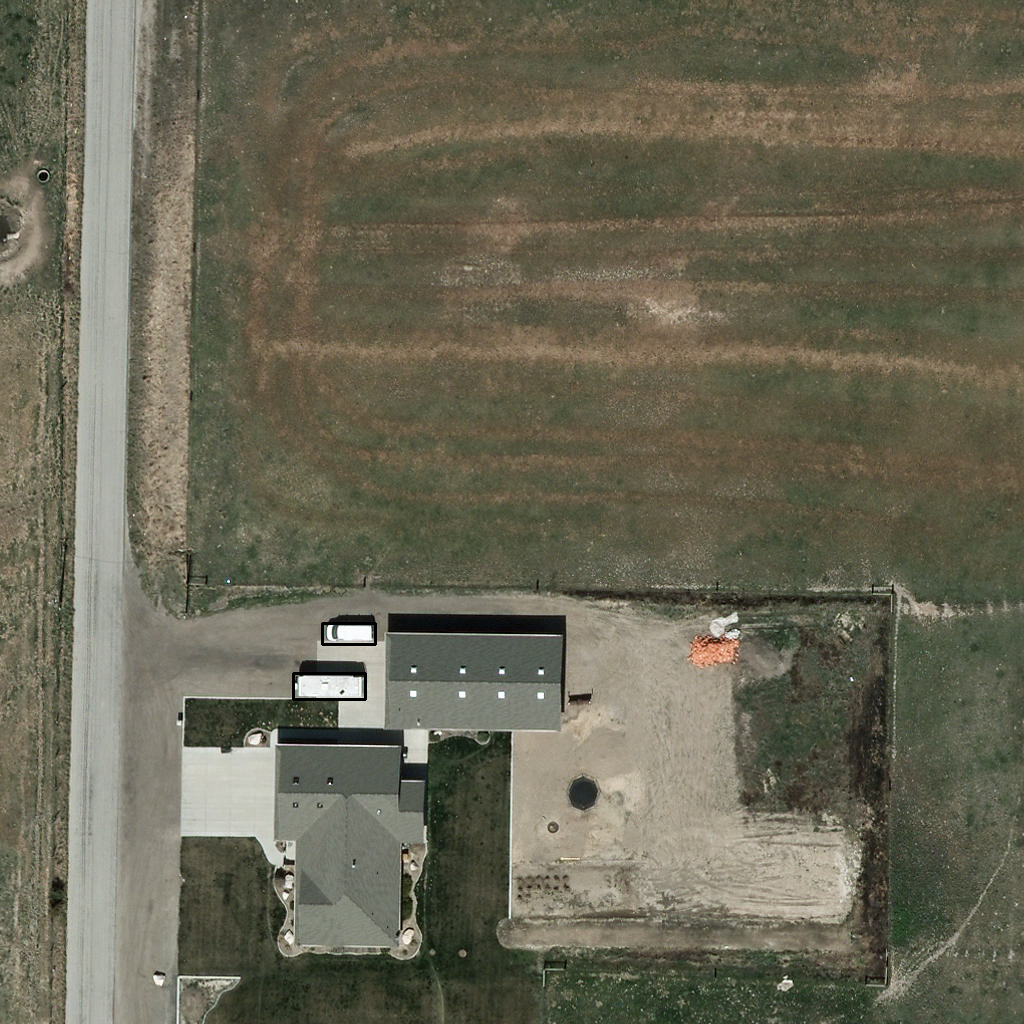
\includegraphics[width=\linewidth]{images/015Results/01abb_vs_obb/comp_images/ground_truth_abb/198.png}
        \caption{Van}
    \end{subfigure}
    \begin{subfigure}[t]{0.38\textwidth}
        \centering
        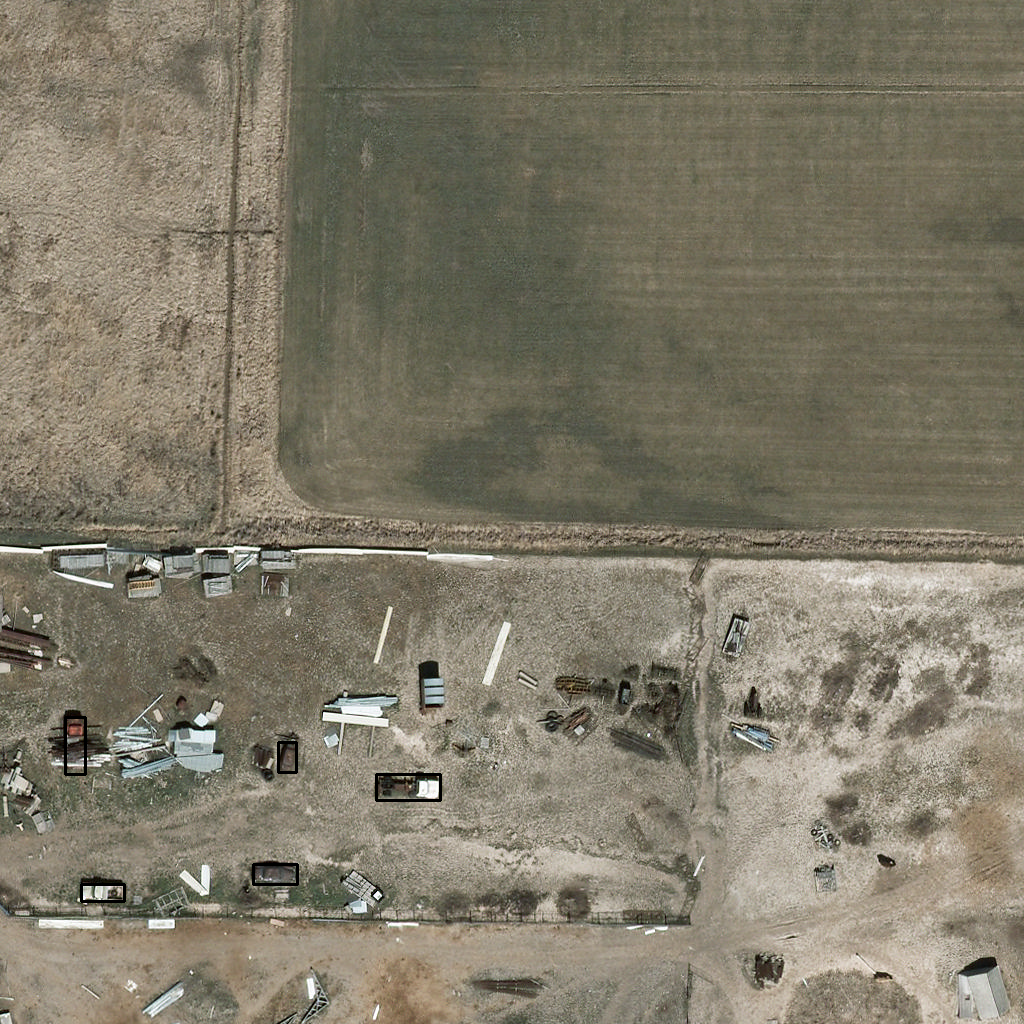
\includegraphics[width=\linewidth]{images/015Results/01abb_vs_obb/comp_images/ground_truth_abb/212.png}
        \caption{Truck}
    \end{subfigure}
    
    \begin{subfigure}[t]{0.38\textwidth}
        \centering
        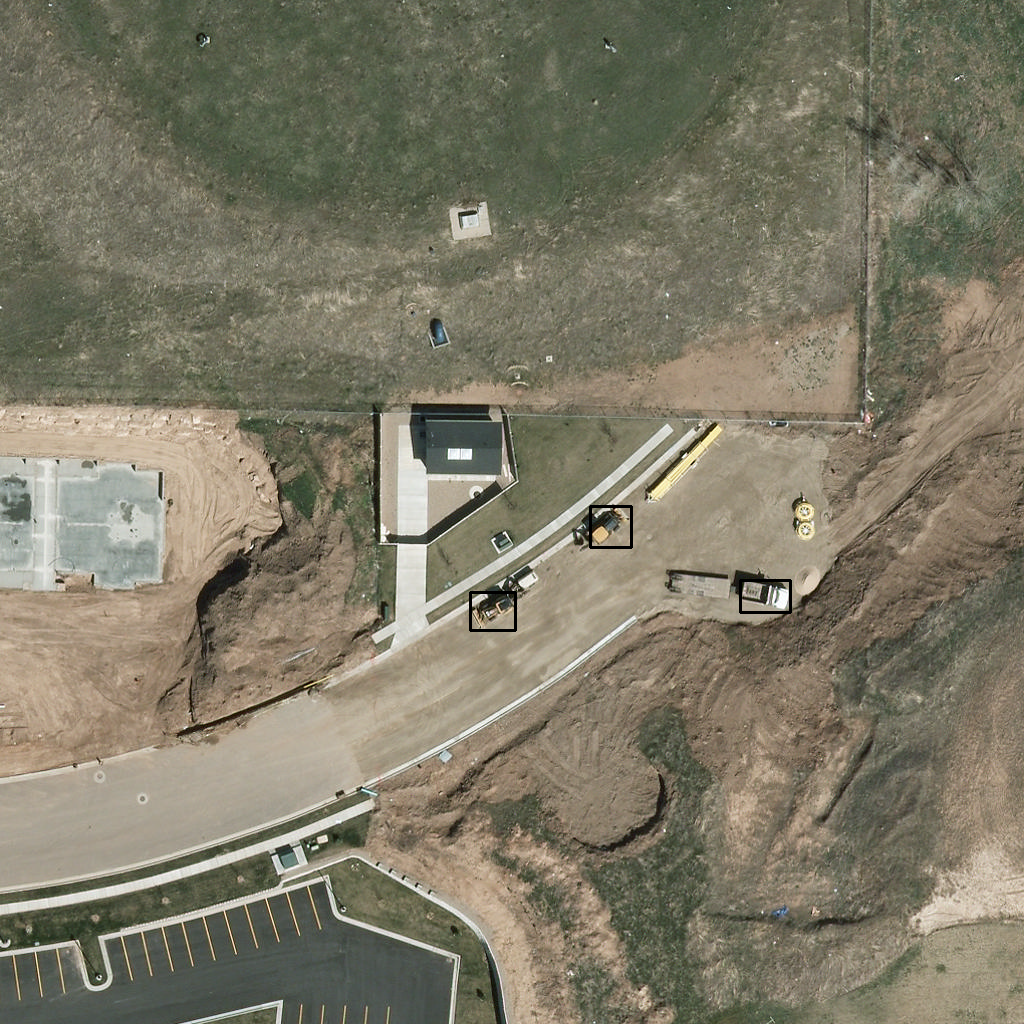
\includegraphics[width=\linewidth]{images/015Results/01abb_vs_obb/comp_images/ground_truth_abb/427.png}
        \caption{Vehicle}
    \end{subfigure}
    \begin{subfigure}[t]{0.38\textwidth}
        \centering
        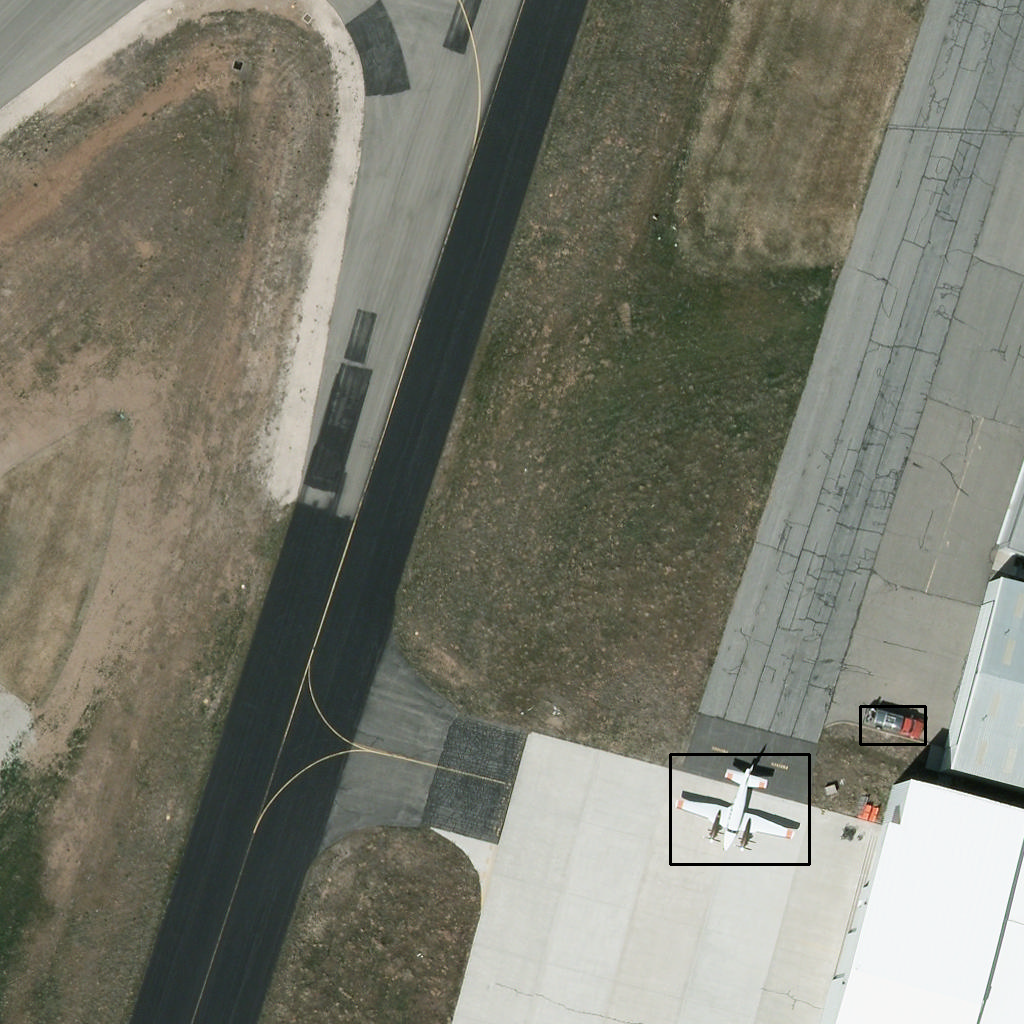
\includegraphics[width=\linewidth]{images/015Results/01abb_vs_obb/comp_images/ground_truth_abb/487.png}
        \caption{Plane}
    \end{subfigure}
    
    \begin{subfigure}[t]{0.38\textwidth}
        \centering
        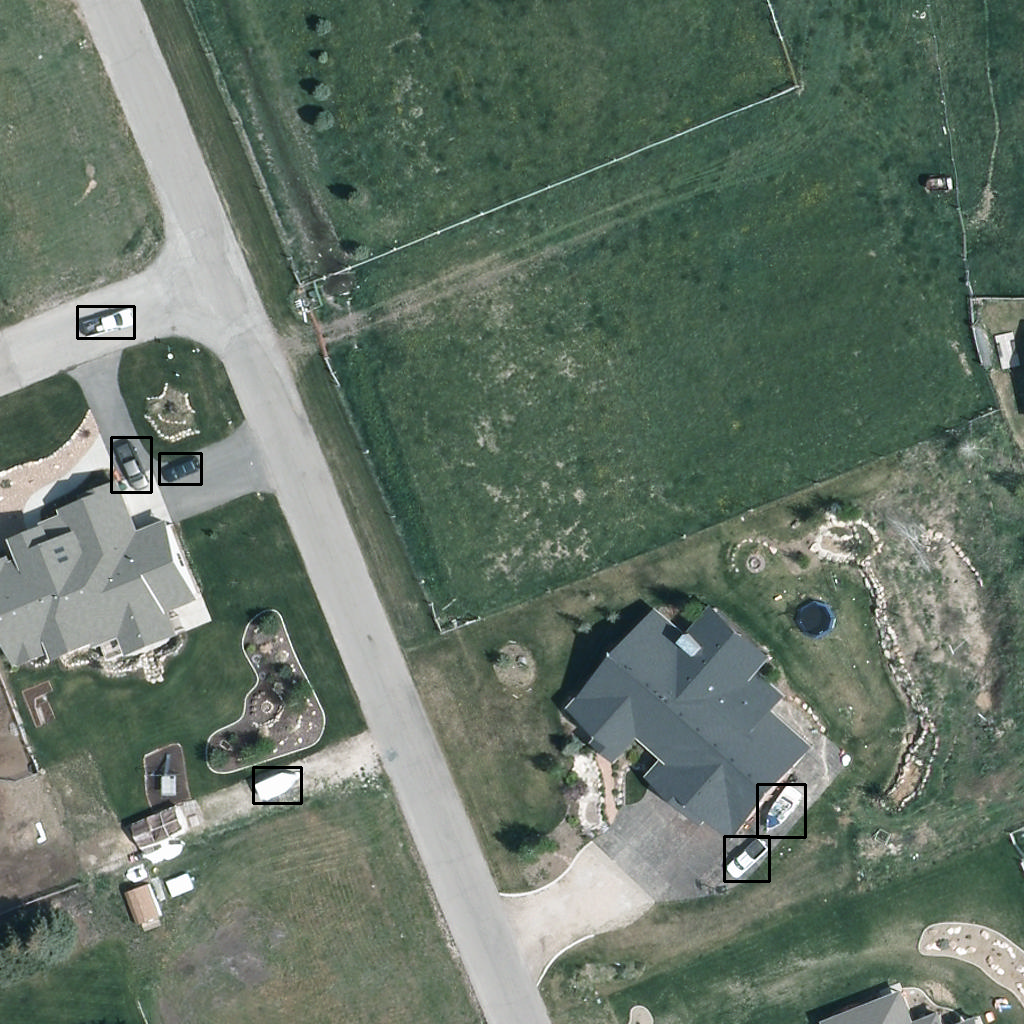
\includegraphics[width=\linewidth]{images/015Results/01abb_vs_obb/comp_images/ground_truth_abb/509.png}
        \caption{Ship}
    \end{subfigure}
    \begin{subfigure}[t]{0.38\textwidth}
        \centering
        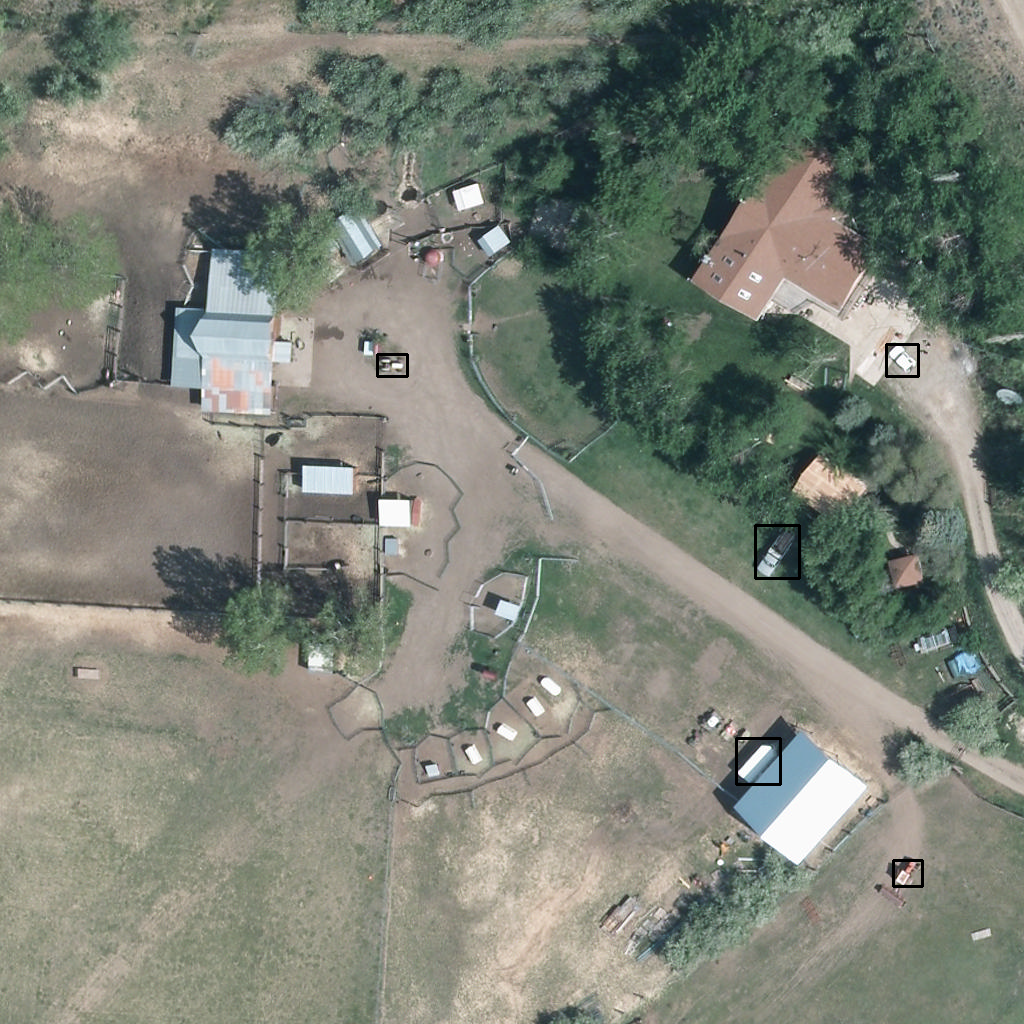
\includegraphics[width=\linewidth]{images/015Results/01abb_vs_obb/comp_images/ground_truth_abb/523.png}
        \caption{Car, Tractor, Pick-Up}
    \end{subfigure}
    
    \caption[Ground Truth (ABB) – Full Sized Images]{Ground Truth (ABB) – Full Sized Images. The captions below the partial illustrations correspond to the classes shown in the example images. However, the illustrations generally show more classes than are indicated in the captions.}
    \label{fig:gt_abb_examples_fs}
\end{figure}



\begin{figure}[h!]
    \centering
    \begin{subfigure}[t]{0.38\textwidth}
        \centering
        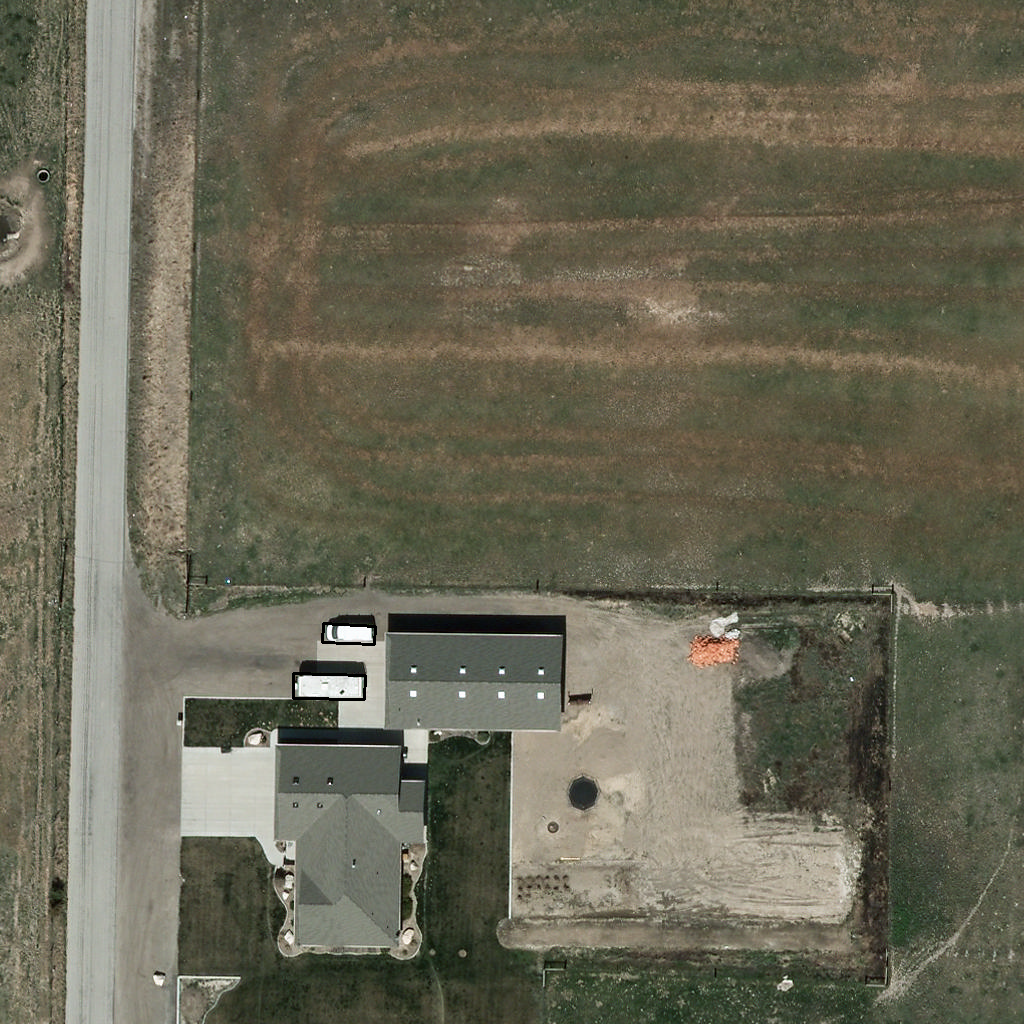
\includegraphics[width=\linewidth]{images/015Results/01abb_vs_obb/comp_images/ground_truth_obb/198.png}
        \caption{Van}
    \end{subfigure}
    \begin{subfigure}[t]{0.38\textwidth}
        \centering
        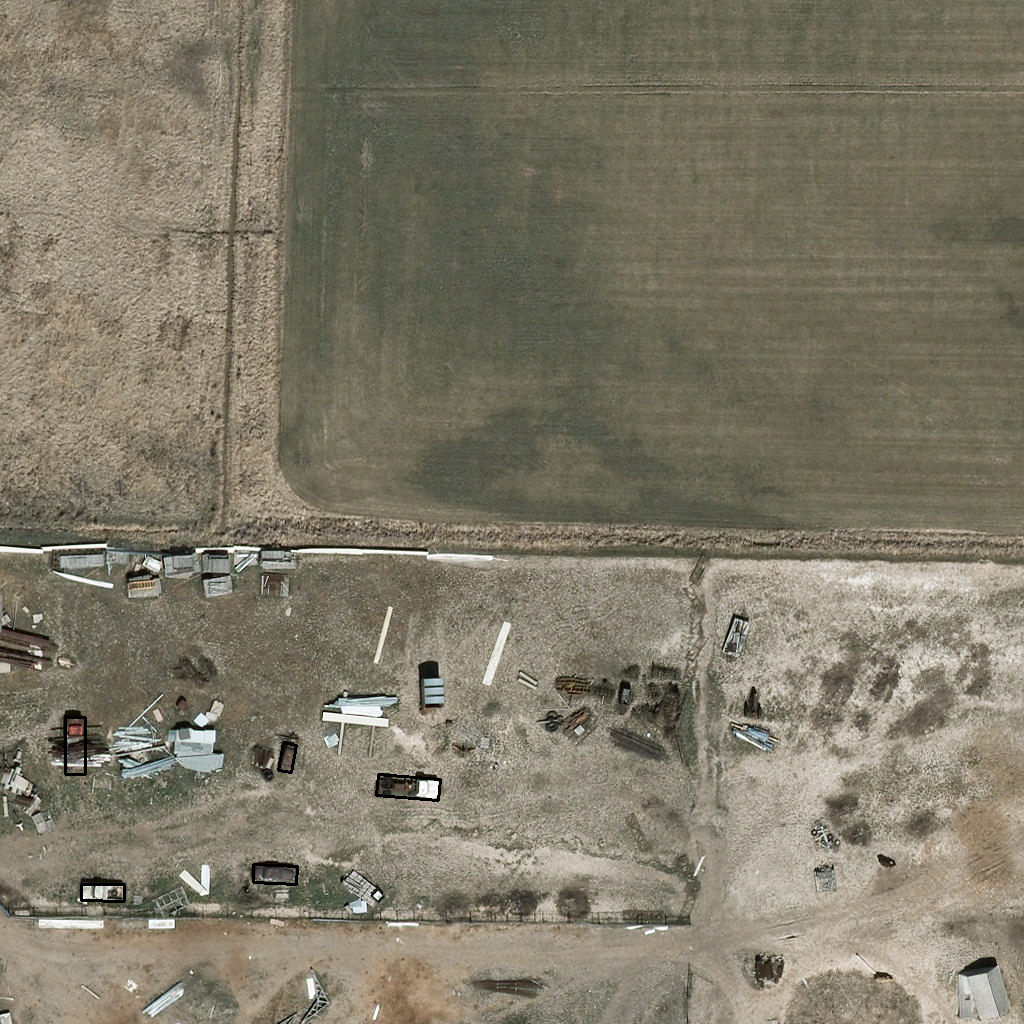
\includegraphics[width=\linewidth]{images/015Results/01abb_vs_obb/comp_images/ground_truth_obb/212.png}
        \caption{Truck}
    \end{subfigure}
    
    \begin{subfigure}[t]{0.38\textwidth}
        \centering
        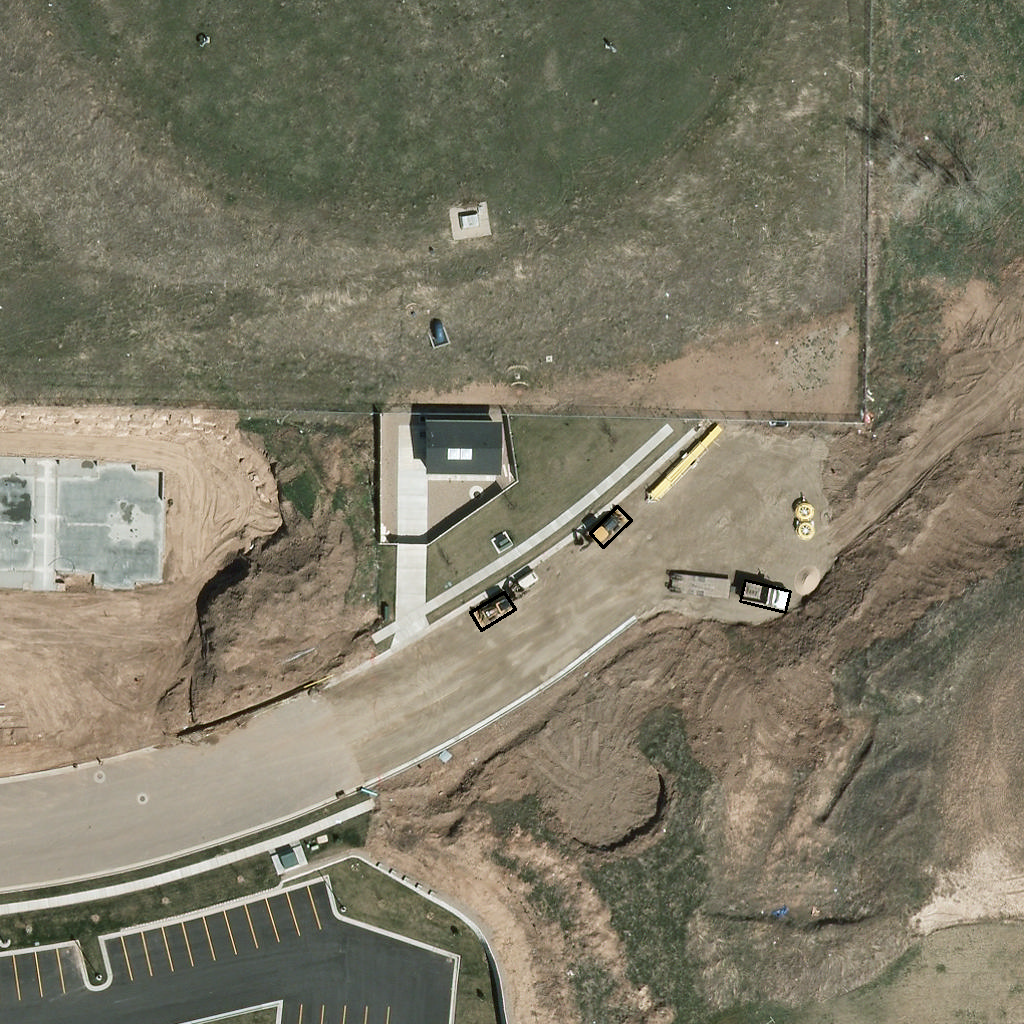
\includegraphics[width=\linewidth]{images/015Results/01abb_vs_obb/comp_images/ground_truth_obb/427.png}
        \caption{Vehicle}
    \end{subfigure}
    \begin{subfigure}[t]{0.38\textwidth}
        \centering
        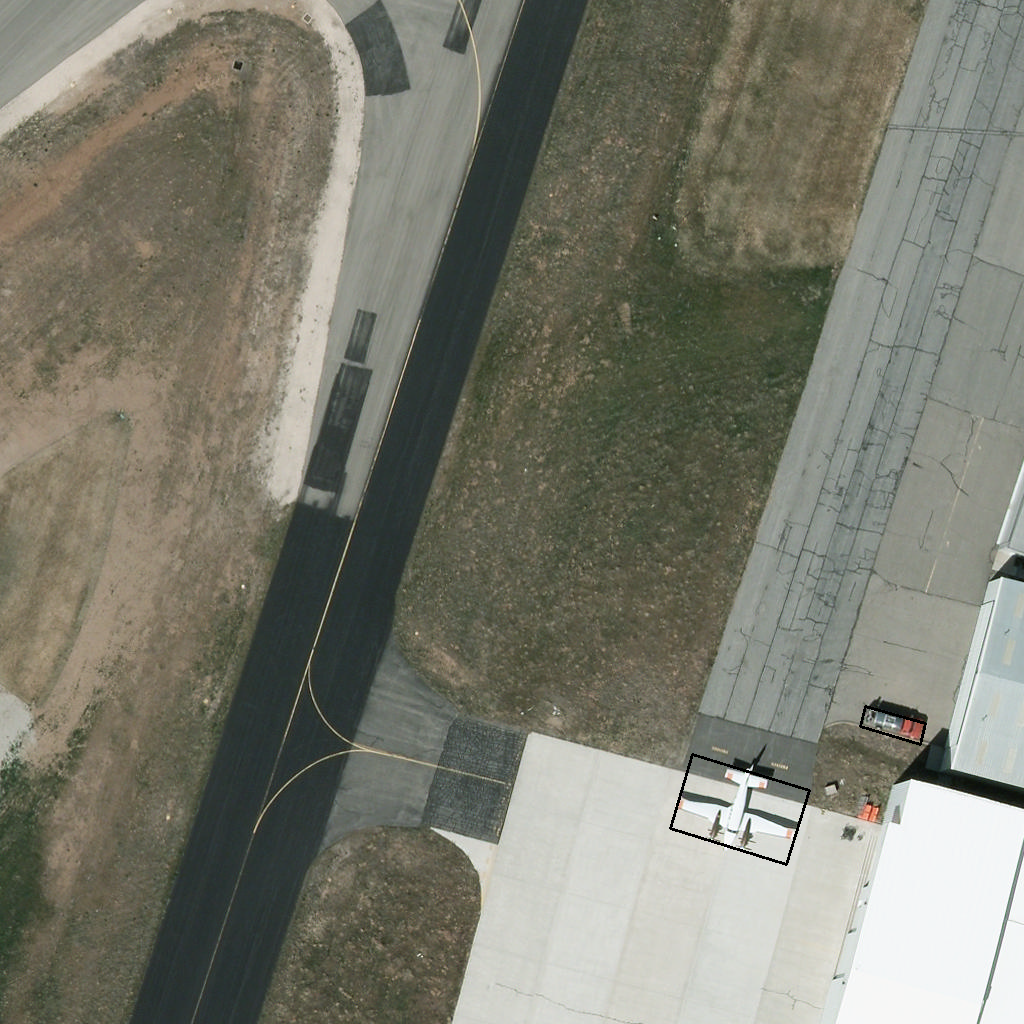
\includegraphics[width=\linewidth]{images/015Results/01abb_vs_obb/comp_images/ground_truth_obb/487.png}
        \caption{Plane}
    \end{subfigure}
    
    \begin{subfigure}[t]{0.38\textwidth}
        \centering
        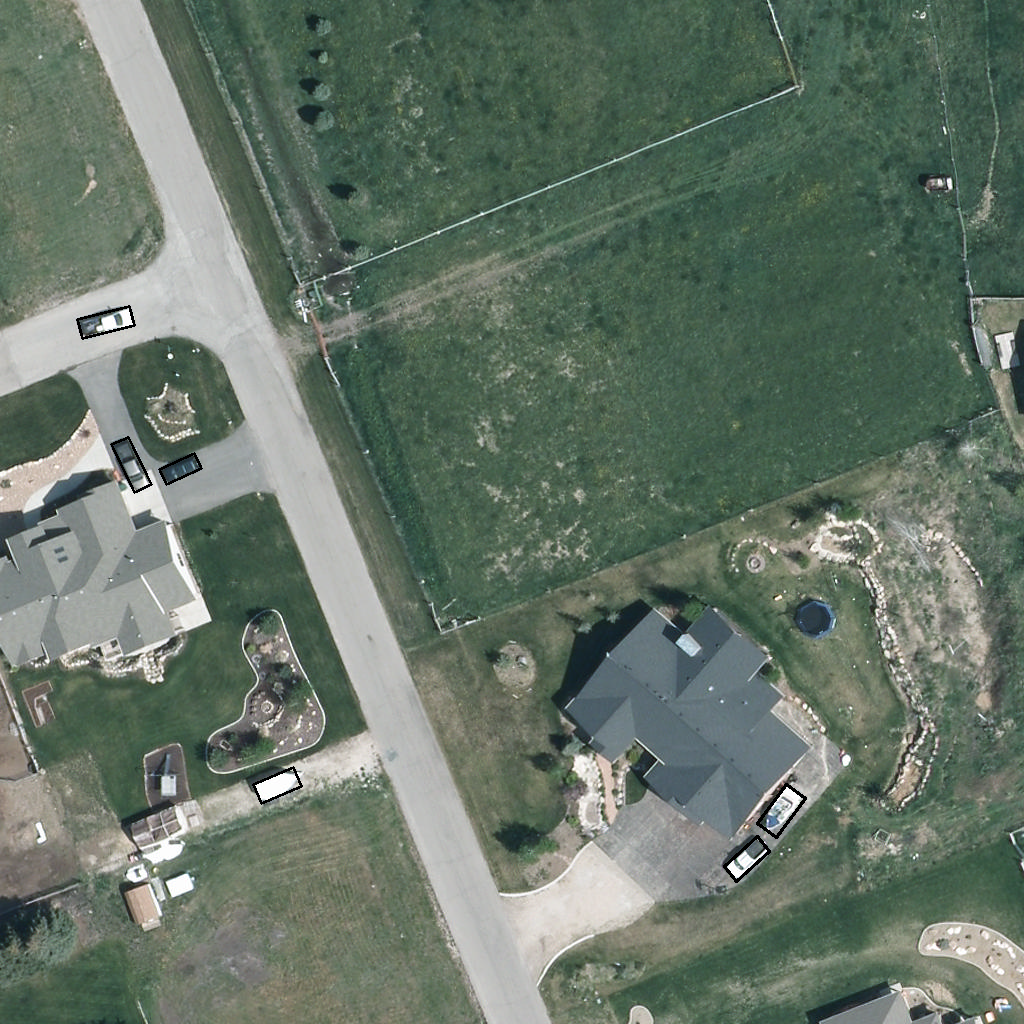
\includegraphics[width=\linewidth]{images/015Results/01abb_vs_obb/comp_images/ground_truth_obb/509.png}
        \caption{Ship}
    \end{subfigure}
    \begin{subfigure}[t]{0.38\textwidth}
        \centering
        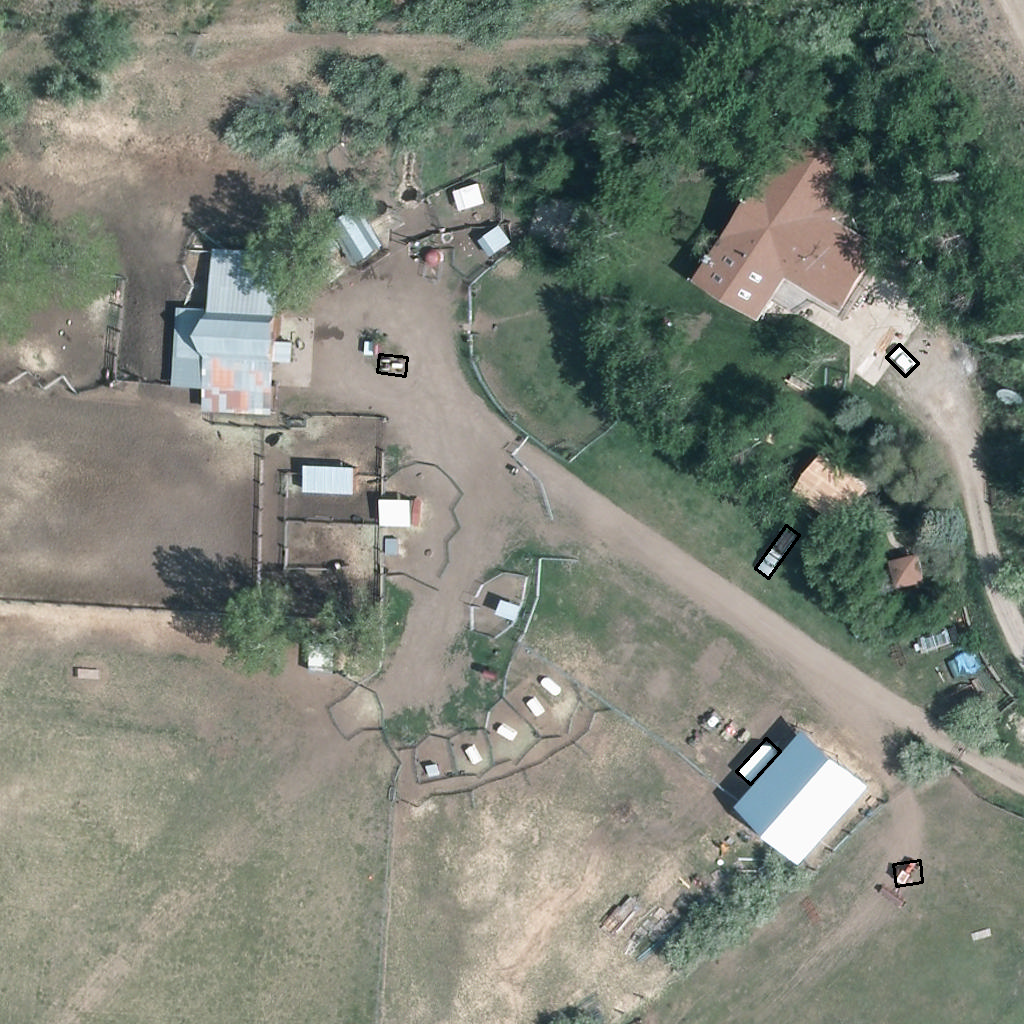
\includegraphics[width=\linewidth]{images/015Results/01abb_vs_obb/comp_images/ground_truth_obb/523.png}
        \caption{Car, Tractor, Pick-Up}
    \end{subfigure}
    
    \caption[Ground Truth (OBB) – Full Sized Images]{Ground Truth (OBB) – Full Sized Images. The captions below the partial illustrations correspond to the classes shown in the example images. However, the illustrations generally show more classes than are indicated in the captions.}
    \label{fig:gt_obb_examples_fs}
\end{figure}




\begin{figure}[h!]
    \centering
    \begin{subfigure}[t]{0.38\textwidth}
        \centering
        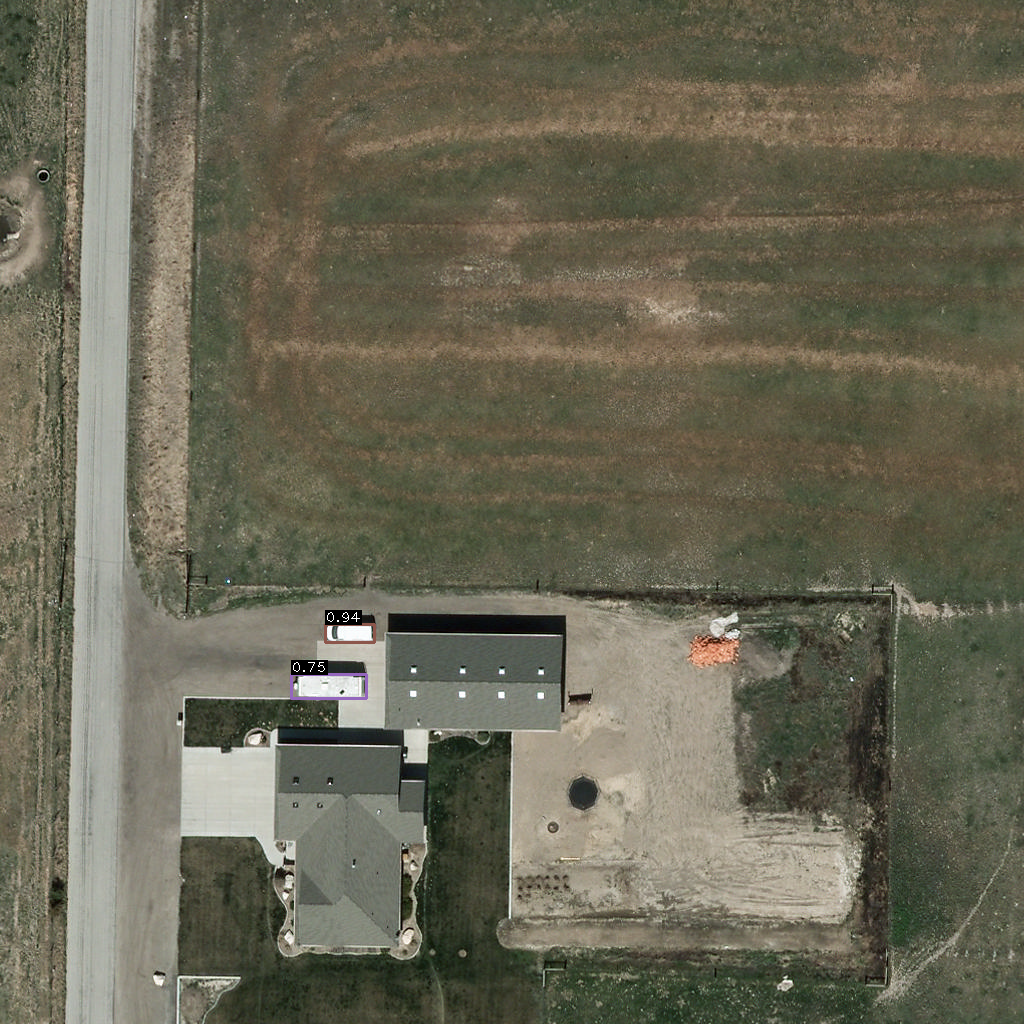
\includegraphics[width=\linewidth]{images/015Results/01abb_vs_obb/comp_images/abb/198.png}
        \caption{Van}
    \end{subfigure}
    \begin{subfigure}[t]{0.38\textwidth}
        \centering
        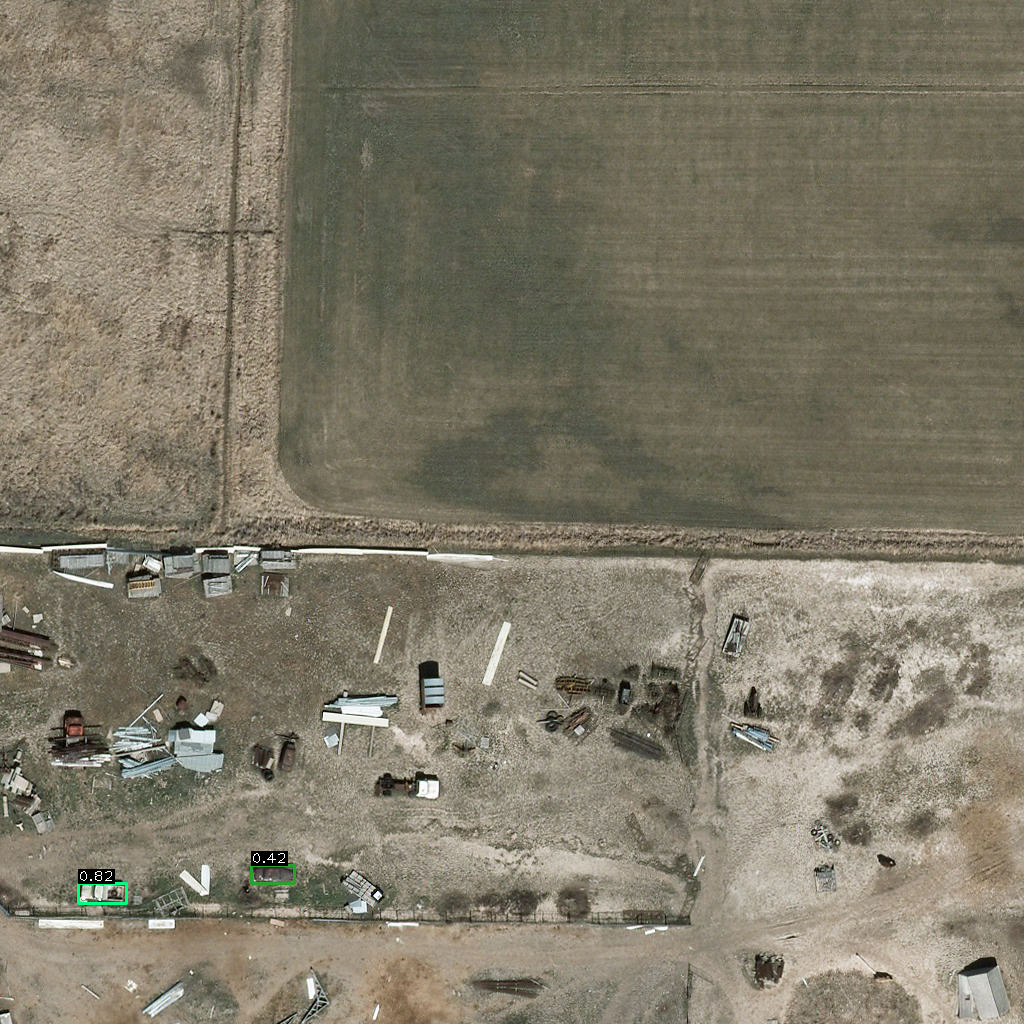
\includegraphics[width=\linewidth]{images/015Results/01abb_vs_obb/comp_images/abb/212.png}
        \caption{Truck}
    \end{subfigure}
    
    \begin{subfigure}[t]{0.38\textwidth}
        \centering
        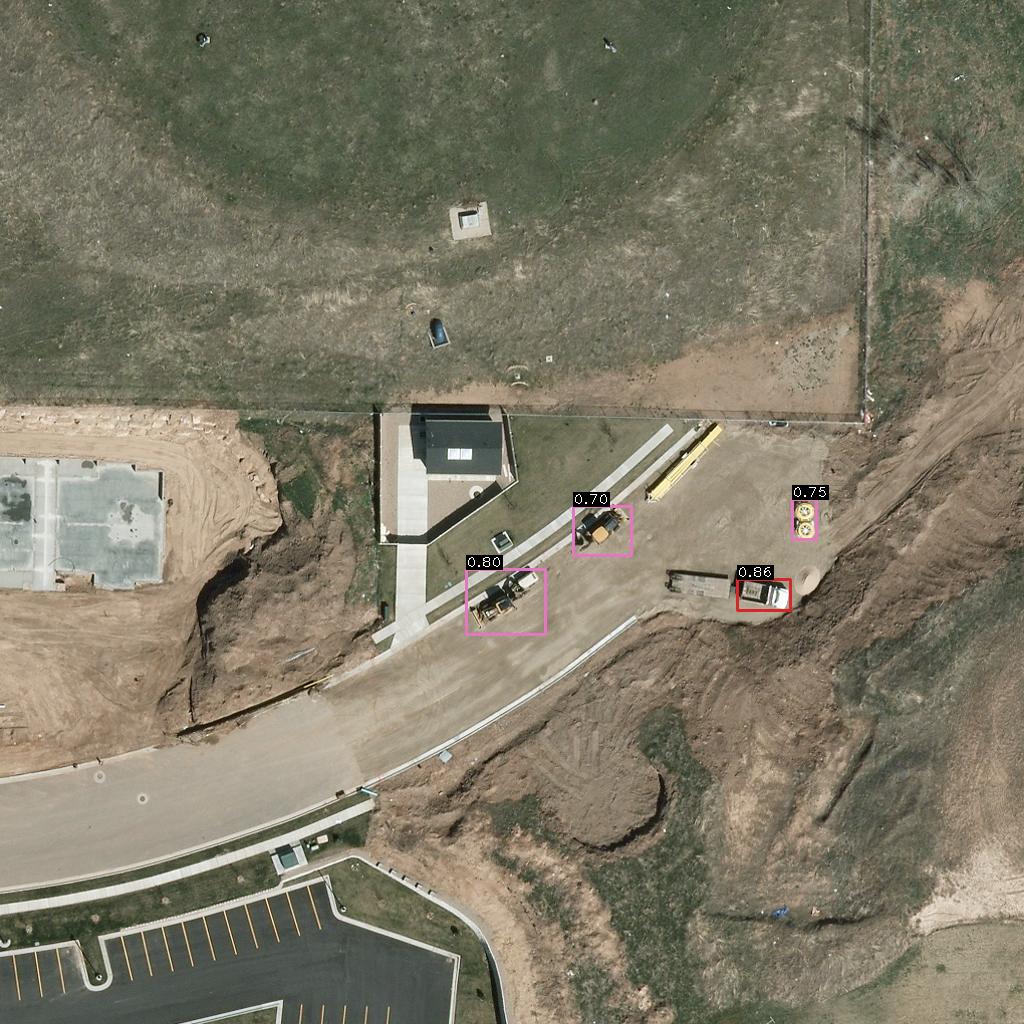
\includegraphics[width=\linewidth]{images/015Results/01abb_vs_obb/comp_images/abb/427.png}
        \caption{Vehicle}
    \end{subfigure}
    \begin{subfigure}[t]{0.38\textwidth}
        \centering
        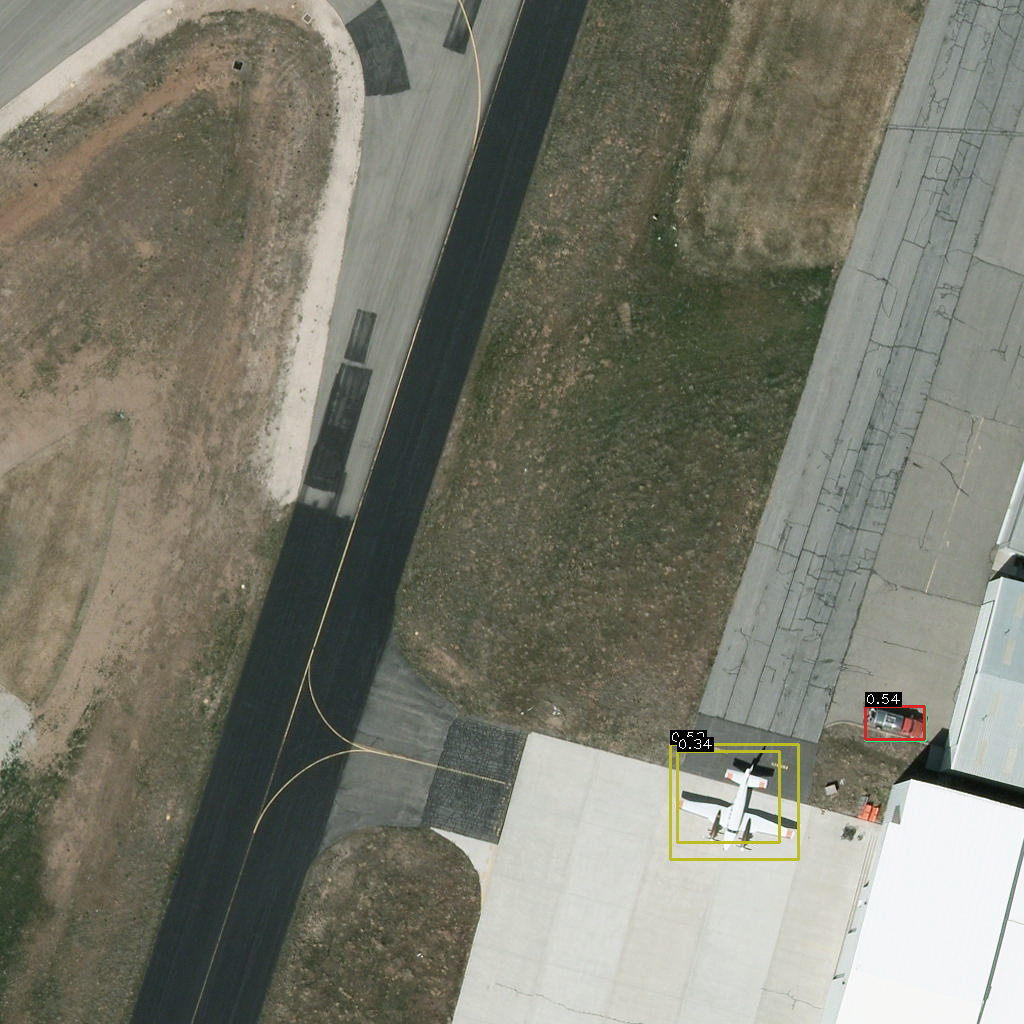
\includegraphics[width=\linewidth]{images/015Results/01abb_vs_obb/comp_images/abb/487.png}
        \caption{Plane}
    \end{subfigure}
    
    \begin{subfigure}[t]{0.38\textwidth}
        \centering
        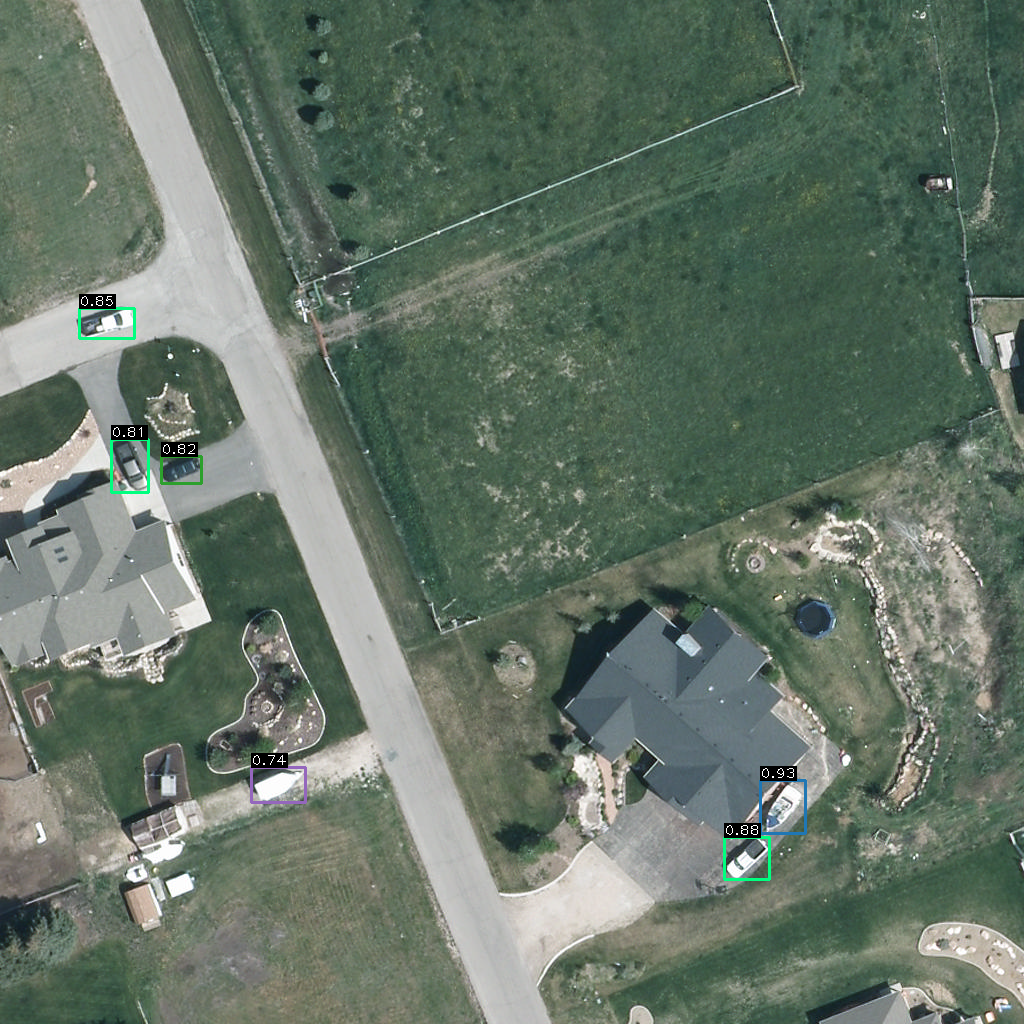
\includegraphics[width=\linewidth]{images/015Results/01abb_vs_obb/comp_images/abb/509.png}
        \caption{Ship}
    \end{subfigure}
    \begin{subfigure}[t]{0.38\textwidth}
        \centering
        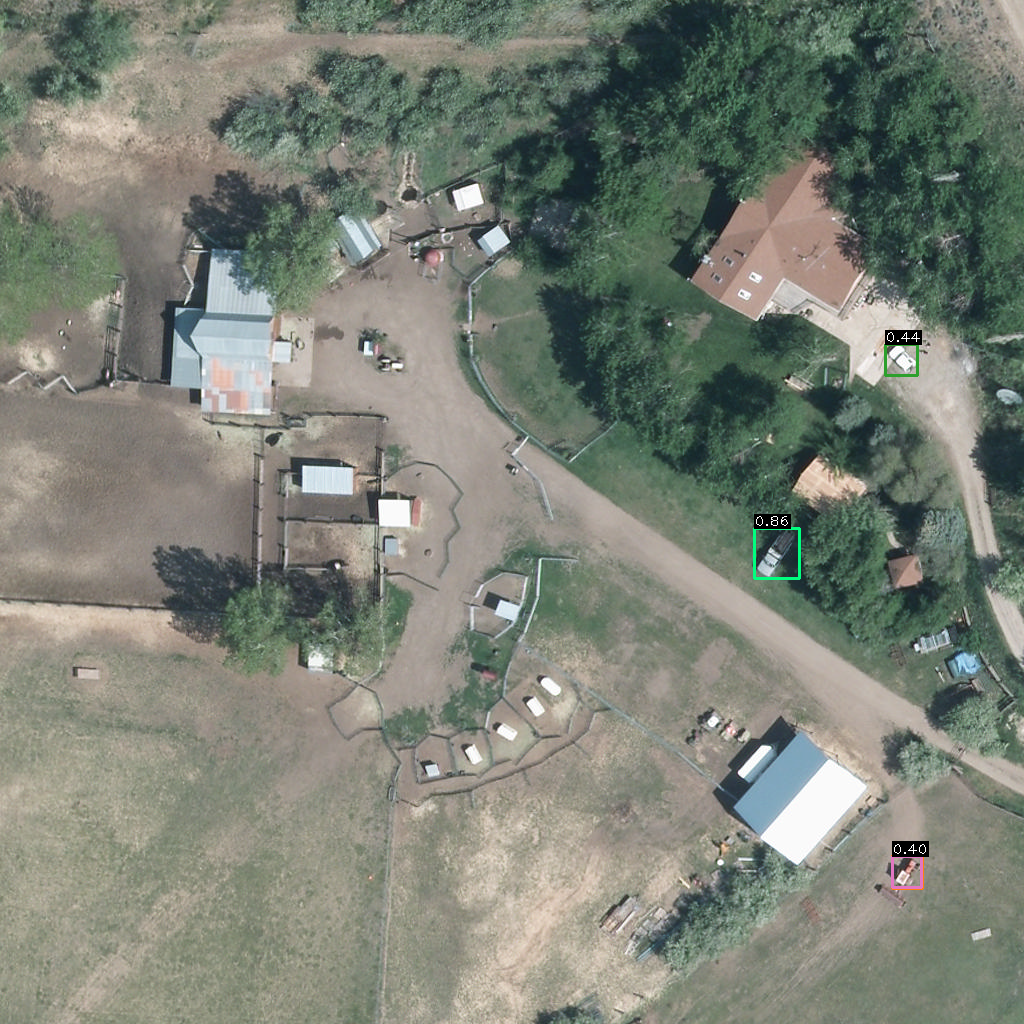
\includegraphics[width=\linewidth]{images/015Results/01abb_vs_obb/comp_images/abb/523.png}
        \caption{Car, Tractor, Pick-Up}
    \end{subfigure}
    
    \caption[ABB Model – Full Sized Images]{ABB Model – Full Sized Images. The captions below the partial illustrations correspond to the classes shown in the example images. However, the illustrations generally show more classes than are indicated in the captions.}
    \label{fig:ABB_examples_fs}
\end{figure}

\begin{figure}[h!]
    \centering
    \begin{subfigure}[t]{0.38\textwidth}
        \centering
        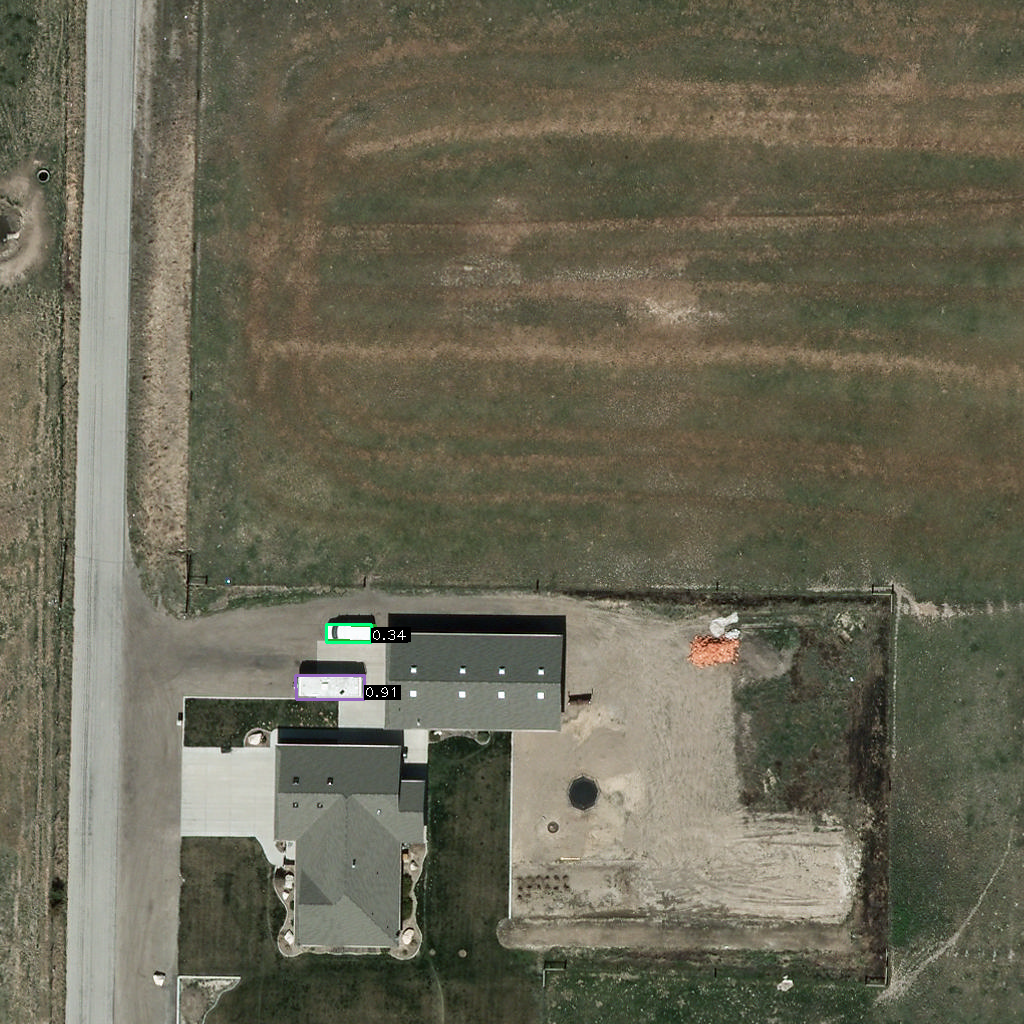
\includegraphics[width=\linewidth]{images/015Results/01abb_vs_obb/comp_images/obb/198.png}
        \caption{Van}
    \end{subfigure}
    \begin{subfigure}[t]{0.38\textwidth}
        \centering
        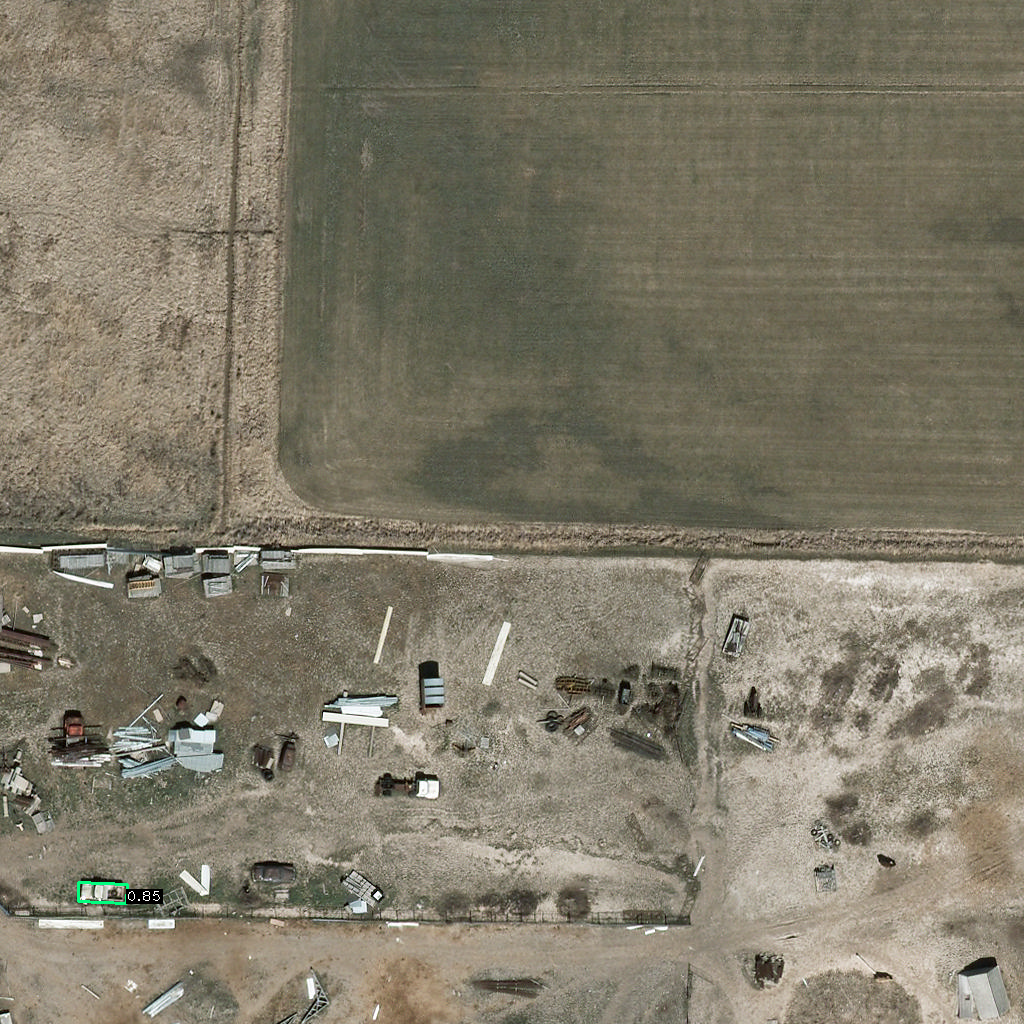
\includegraphics[width=\linewidth]{images/015Results/01abb_vs_obb/comp_images/obb/212.png}
        \caption{Truck}
    \end{subfigure}
    
    \begin{subfigure}[t]{0.38\textwidth}
        \centering
        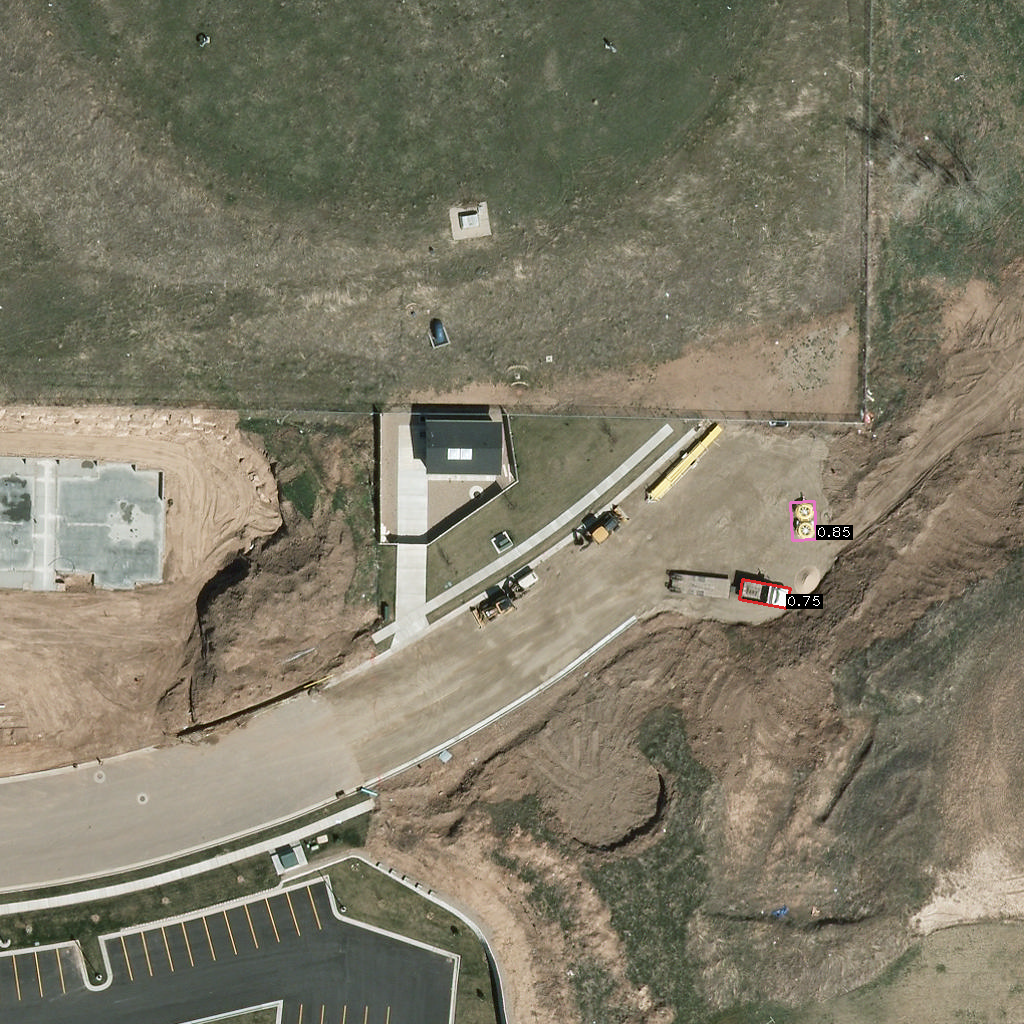
\includegraphics[width=\linewidth]{images/015Results/01abb_vs_obb/comp_images/obb/427.png}
        \caption{Vehicle}
    \end{subfigure}
    \begin{subfigure}[t]{0.38\textwidth}
        \centering
        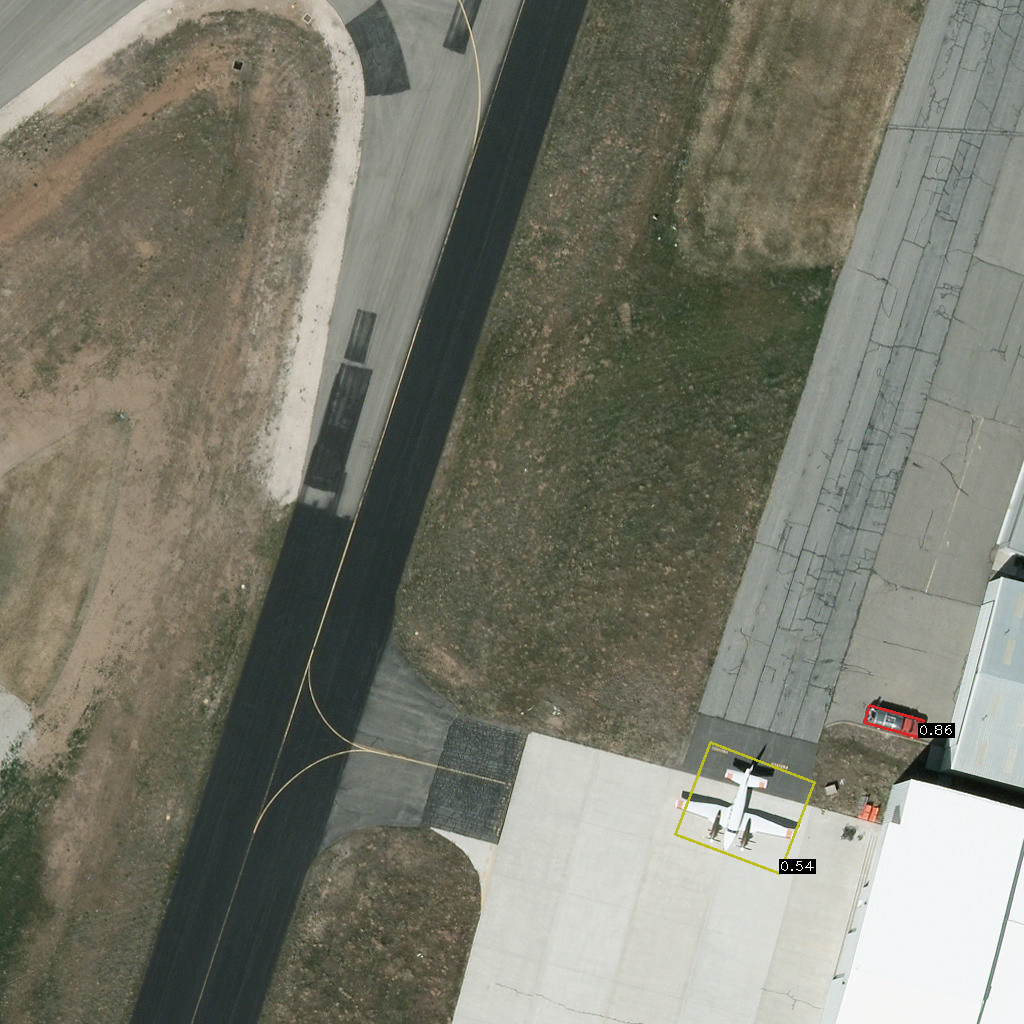
\includegraphics[width=\linewidth]{images/015Results/01abb_vs_obb/comp_images/obb/487.png}
        \caption{Plane}
    \end{subfigure}
    
    \begin{subfigure}[t]{0.38\textwidth}
        \centering
        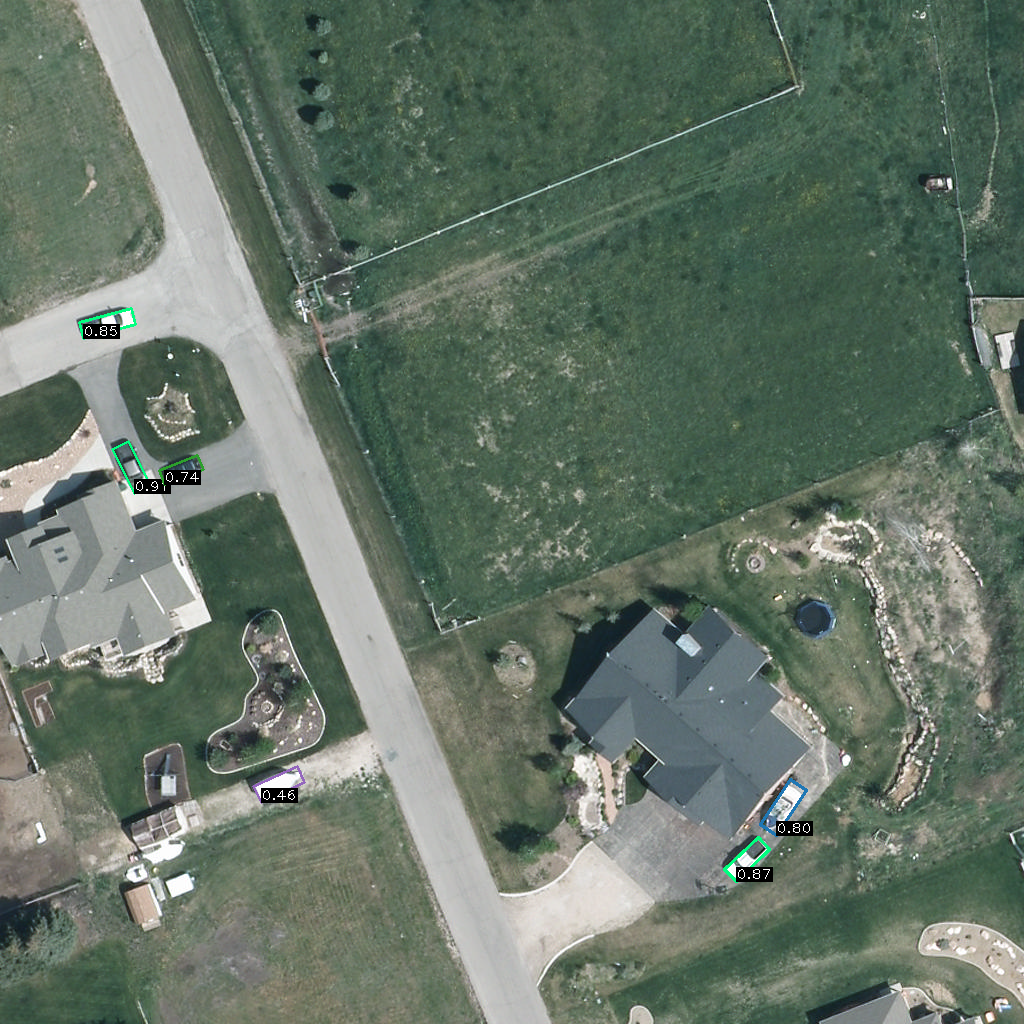
\includegraphics[width=\linewidth]{images/015Results/01abb_vs_obb/comp_images/obb/509.png}
        \caption{Ship}
    \end{subfigure}
    \begin{subfigure}[t]{0.38\textwidth}
        \centering
        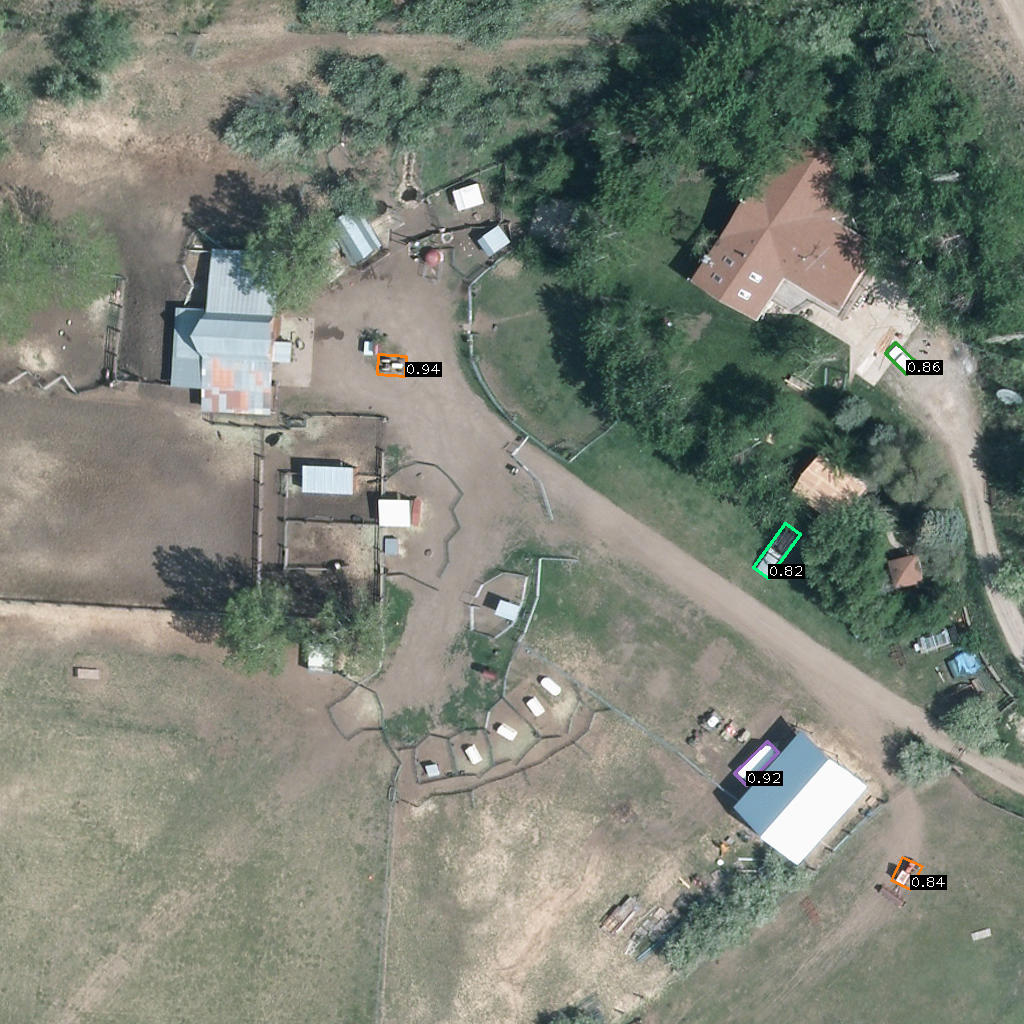
\includegraphics[width=\linewidth]{images/015Results/01abb_vs_obb/comp_images/obb/523.png}
        \caption{Car, Tractor, Pick-Up}
    \end{subfigure}
    
    \caption[OBB Model – Full Sized Images]{OBB Model – Full Sized Images. The captions below the partial illustrations correspond to the classes shown in the example images. However, the illustrations generally show more classes than are indicated in the captions.}
    \label{fig:OBB_examples_fs}
\end{figure}



\begin{figure}[h!]
    \centering
    \begin{subfigure}[t]{0.38\textwidth}
        \centering
        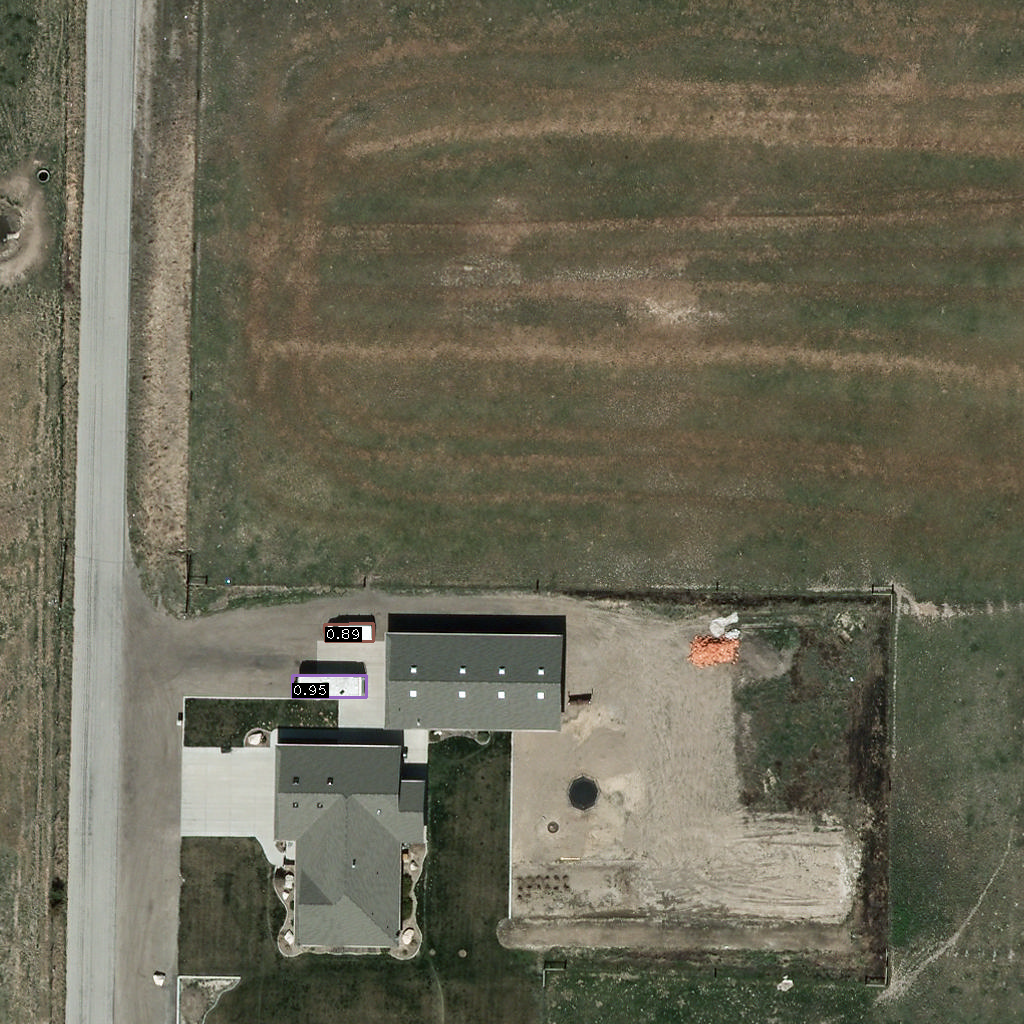
\includegraphics[width=\linewidth]{images/015Results/01abb_vs_obb/comp_images/aab_old/198.png}
        \caption{Van}
    \end{subfigure}
    \begin{subfigure}[t]{0.38\textwidth}
        \centering
        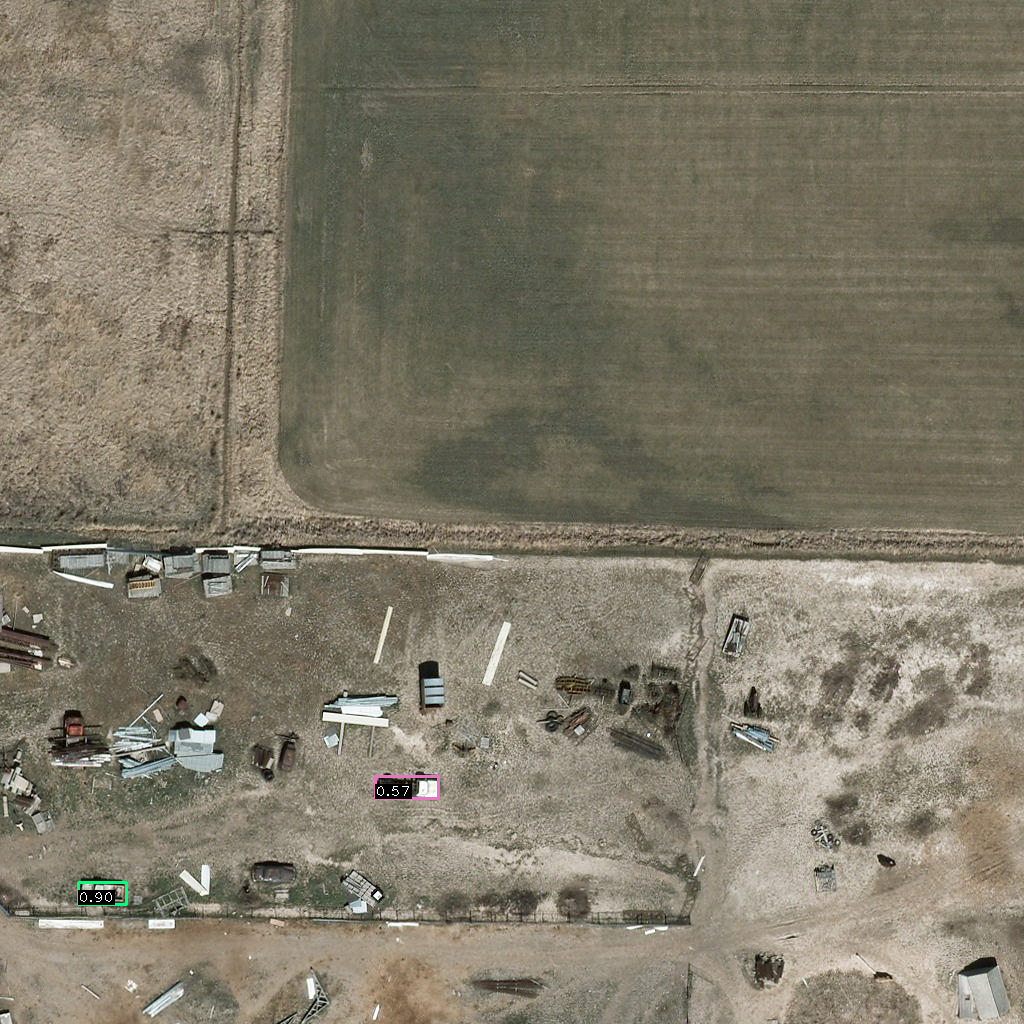
\includegraphics[width=\linewidth]{images/015Results/01abb_vs_obb/comp_images/aab_old/212.png}
        \caption{Truck}
    \end{subfigure}
    
    \begin{subfigure}[t]{0.38\textwidth}
        \centering
        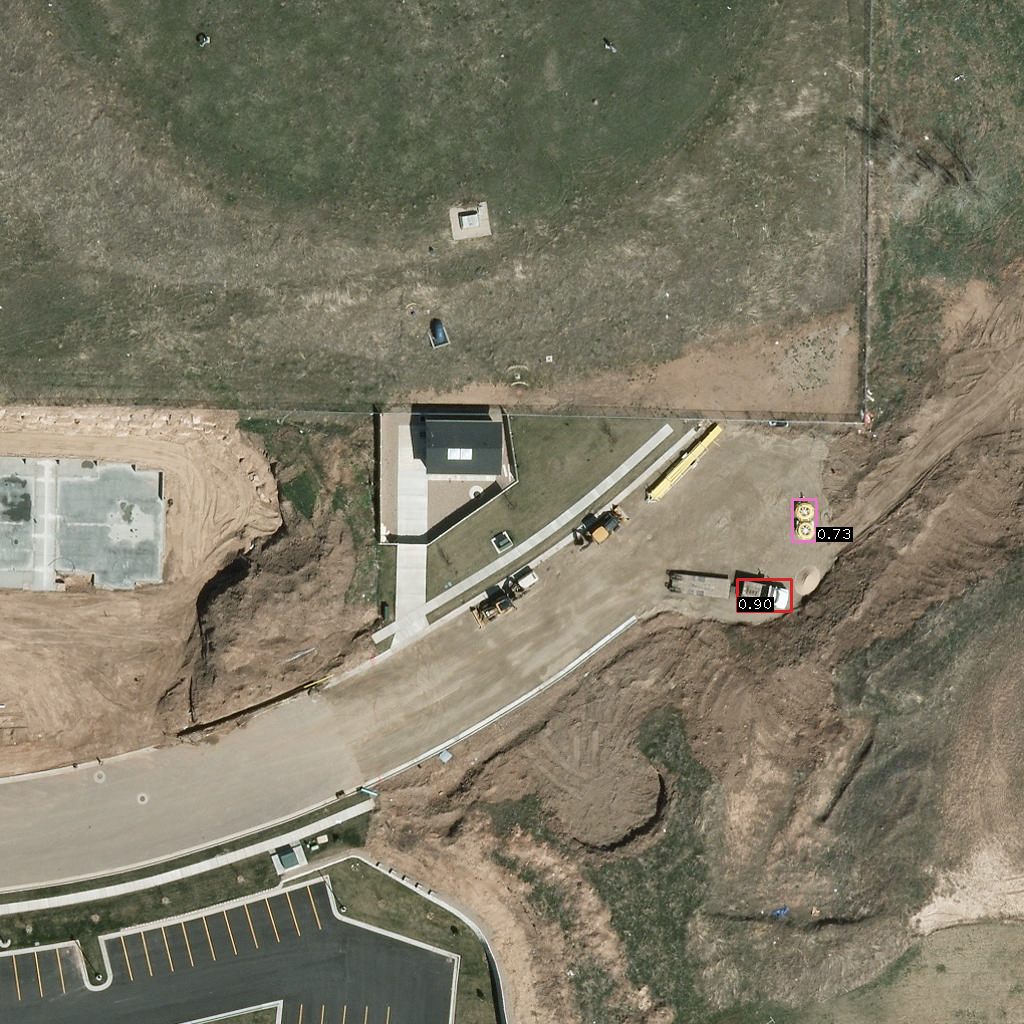
\includegraphics[width=\linewidth]{images/015Results/01abb_vs_obb/comp_images/aab_old/427.png}
        \caption{Vehicle}
    \end{subfigure}
    \begin{subfigure}[t]{0.38\textwidth}
        \centering
        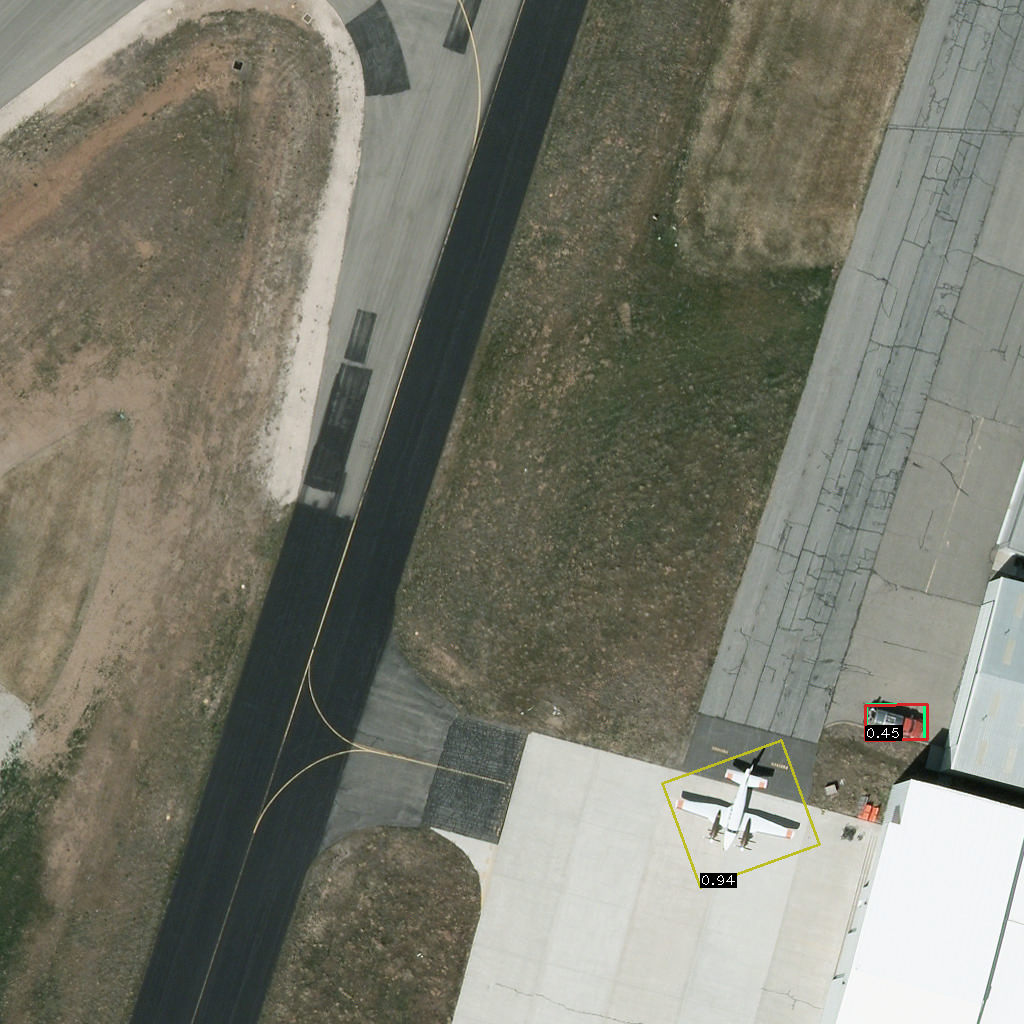
\includegraphics[width=\linewidth]{images/015Results/01abb_vs_obb/comp_images/aab_old/487.png}
        \caption{Plane}
    \end{subfigure}
    
    \begin{subfigure}[t]{0.38\textwidth}
        \centering
        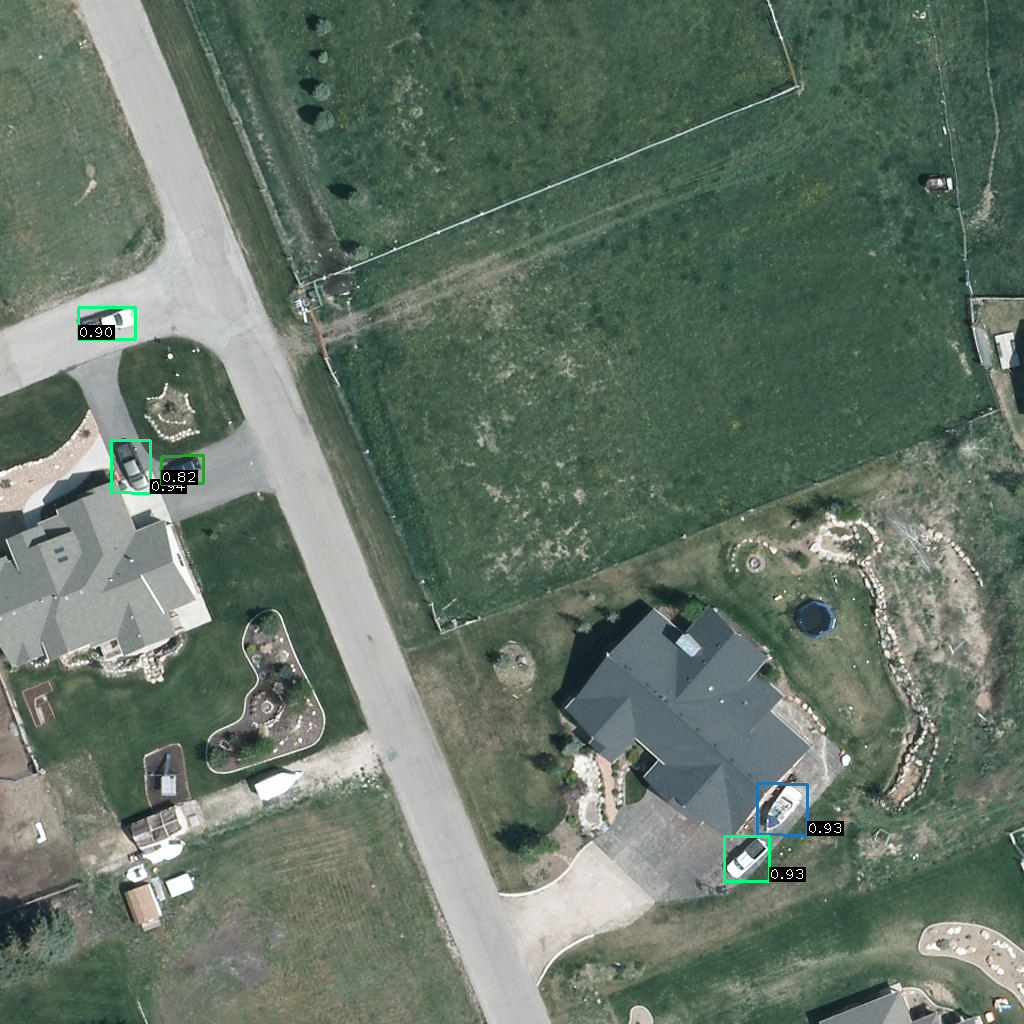
\includegraphics[width=\linewidth]{images/015Results/01abb_vs_obb/comp_images/aab_old/509.png}
        \caption{Ship}
    \end{subfigure}
    \begin{subfigure}[t]{0.38\textwidth}
        \centering
        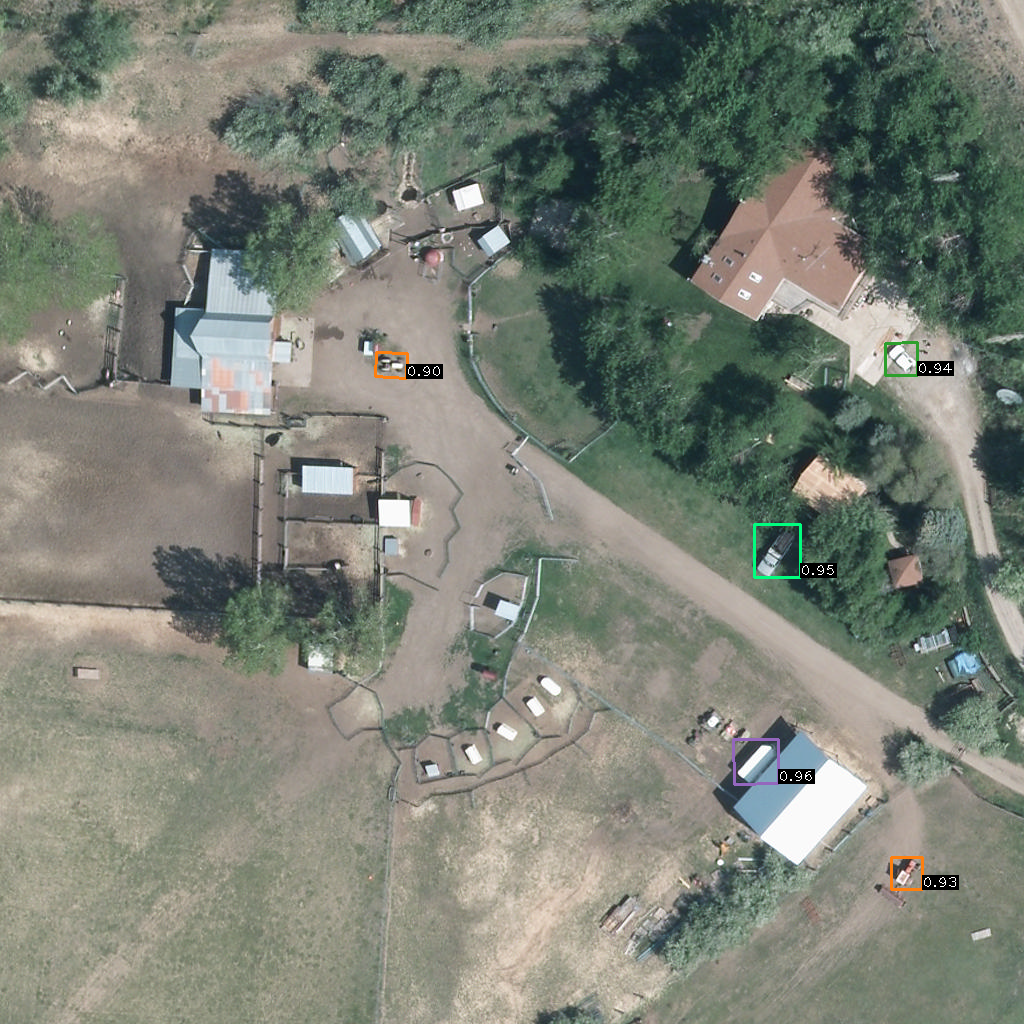
\includegraphics[width=\linewidth]{images/015Results/01abb_vs_obb/comp_images/aab_old/523.png}
        \caption{Car, Tractor, Pick-Up}
    \end{subfigure}
    
    \caption["ABB in OBB" Model – Full Sized Images]{"ABB in OBB" Model – Full Sized Images. The captions below the partial illustrations correspond to the classes shown in the example images. However, the illustrations generally show more classes than are indicated in the captions.}
    \label{fig:ABBinOBB_examples_fs}
\end{figure}